\subsection{Story Designer}

% Me he tomado la libertad de darle el nombre de Story Designer a esta nueva herramienta en EDD. Te parece? Sobre todo es para simplificar cómo nos referimos a él

% \begin{figure*}[t!]
%     \centering
%     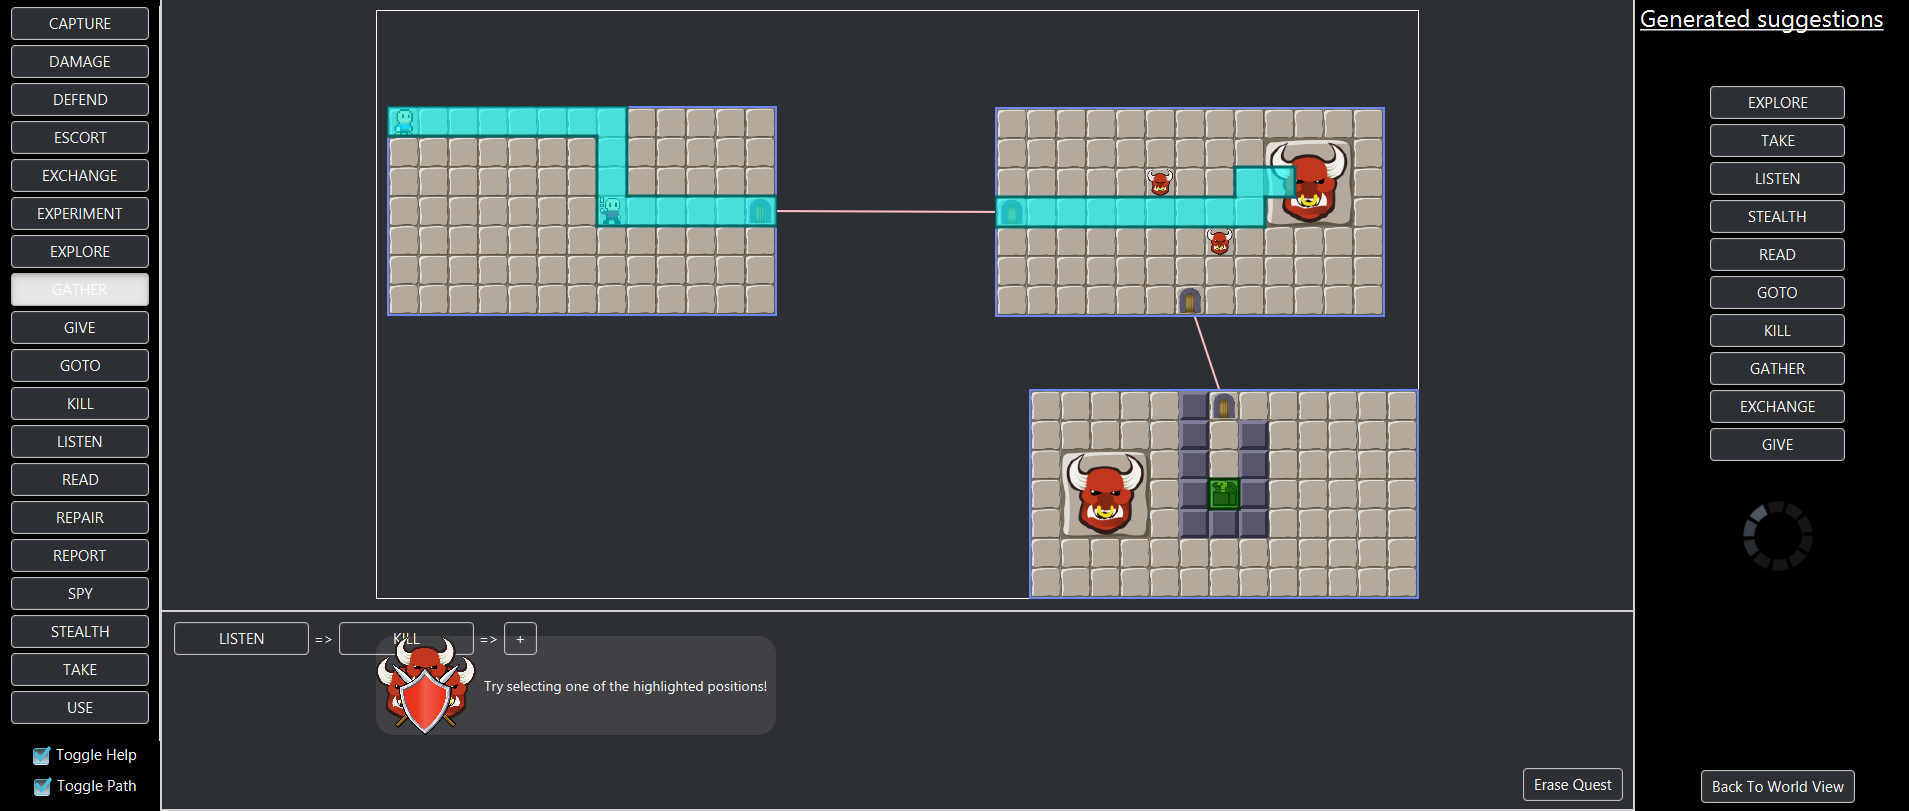
\includegraphics[width=\textwidth]{figures/main-help.png} %temp
%     \caption{The Story Designer screen in EDD.}
%     \label{fig:story-screen}
% \end{figure*}

% \begin{itemize}
% \item Brief intro to the tool's purpose. %done
% \item Subsection about story structures with TVtropes, node types, connection types, examples %done
% \item Subsection with EDD's story structure creation view. %done
% \item Subsection with representing and evolving with Graph Grammars in EDD 
% \end{itemize}

% \begin{table*}[ht]
% \centering
\caption{General consensus on EDD's features} \label{p1tab:consensus}
\resizebox{0.8\textwidth}{!}{
\begin{tabularx}{\textwidth}{|p{0.2\textwidth}|p{0.99\textwidth}|}
\cline{1-2}

Description & Participants’ Consensus \\\cline{1-2}
World Grid  of the dungeon                   & Its purpose of establishing an illusion of a fully realized dungeon is somewhat achieved. However, limitations exist with how it defines feasibility, a dungeon’s starting point, and the entrances, which disrupts the designers’ decisions.                                                                                                                                                                                   \\\cline{1-2}
World View                                  & The world view’s usefulness for the most part could not be established, other than for the purpose of going to the suggestions view (which was already seldom during the user study) and having a closer look at the entire dungeon without any distractions. Some participants preferred features to be already in the room view’s minimap, and some wanted to see more specific functionalities within the world view itself. \\\cline{1-2}

Enabling and  \newline disabling rooms                & As the user study restricted participants to create 3x3 dungeons, this feature for the most part has been neglected. This is also in part because of its accessibility only being in the world view, which proved to be an inefficient view in general. However, its use for bigger dungeon sizes later on was appreciated, especially for more intricate design purposes.                                                      \\\cline{1-2}
Suggestions View                            & Similarly to enabling and disabling rooms, it was quite difficult to encourage the use of this functionality due to the world view’s inefficient usability. However, this could also be due to the dungeon’s small size, as some participants expressed high interest in using more suggestions with larger dungeon sizes.                                                                                                      \\\cline{1-2}
Minimap  \newline  navigation                      & The minimap proved to be a strong tool not only for navigation purposes, but also for supporting design decisions and choices. The directional buttons were rarely used, but their room previews were helpful in emphasizing the current room’s connection to adjacent rooms without looking at the minimap. On the other hand, this lowered the usability of the world view.                                                   \\\cline{1-2}
Parameters                                       & The parameters were, in general, lacking. They served to be important in decision-making when choosing a suggested map in room view, but there were still doubts on their accuracy and sufficiency when providing information about the generated suggestions.                                                                                                                                                                       \\\cline{1-2}
Generated maps for  \newline  suggestions in room view & Suggestions in the room view proved to be very helpful in supporting the whole design process as they primarily acted as inspirations for the users. The most prominent comment among the users is the preference of having more control on how suggestions should be generated depending on different types of parameters.                                                                                                     \\\cline{1-2}
Design \newline  patterns& The patterns’ visualization was, in general, lacking and not self-explanatory. Some participants have expressed interest in using patterns as a parameter in the generation of suggestions.                                                                                                                                                                                                                                     \\\cline{1-2}
Dark theme                                  & EDD’s dark theme for the user interface received a positive response as it makes working with the program easier.
	\\ \cline{1-2}
\end{tabularx}
}
\end{table*}

% \begin{table}
% \begin{center}
% {\caption{Best performing setups based on their internal validation and visualization of clustered data points.}\label{table:setups}}
% \resizebox{\textwidth}{!}{
% \begin{tabular}{ccccccc}
% \hline
% \rule{0pt}{12pt}
% Algorithm&Data&K&$\Diamond$&$\Box$&$\bigtriangleup$ 
% \\ 
% \hline
% \\[-6pt]
% K-Means & Tiles-PCA & 9 & 0.43 & 0.73 & 9438.233 \\ 
% K-Means & Tiles-PCA & 12 & 0.41 & 0.77 & 9436.928 \\
% K-Means & Dimensions-PCA & 12 & 0.43 & 0.73 & 7738.343 \\
% Agglomerative single & Combined-PCA & 6 & 0.51 & 0.43  & 38.833 \\ 
% Agglomerative avg. & Dimensions-PCA & 6 & 0.44 & 0.67 & 3463.567 \\ 
% \hline
% \\[-6pt]
% \multicolumn{6}{l}{$\Diamond$ Silhouette Score\ \
% $\Box$ Davies Bouldin Index\ \
% $\bigtriangleup$ Calinski-Harabasz Index}
% \end{tabular}
% }\end{center}
% \end{table}

% \begin{itemize}
%     \item Brief intro to the tool's purpose.
%     \item Subsection about TropeTwist briefly explaining how tropes are used and the trope patterns. story structures with TVtropes, node types, connection types, examples done \checkmark
%     \item Subsection with EDD's story structure creation view, and workflow. \checkmark
%     \item Add info on the development from questgram with specific NPCs and the questview changed (although, that last part is not relevant). Also add the info on how to actually use this system.
%     \item Brief subsection with how graph gramamrs work and how we represent these graphs for the EA. Not super in detail because all of that is from tropetwist. 
%     \item The things that are extended in this version is the amount of dimensions, and how the elites are shown! (besides actually showing all of this!)
%     \item Dimensions should be addressed in the final subsection. 
%     \item How elites are shown and all of that goes to the workflow subsection.
% \end{itemize}


%\begin{figure*}[t!]
%    \centering
%    \includegraphics[width=\textwidth]{figures/current_GUI.png}
%    \caption{The Story Designer screen in EDD.}
%    \label{fig:story-screen}
%\end{figure*}
 
% \begin{table*}[ht]
% \centering
\caption{General consensus on EDD's features} \label{p1tab:consensus}
\resizebox{0.8\textwidth}{!}{
\begin{tabularx}{\textwidth}{|p{0.2\textwidth}|p{0.99\textwidth}|}
\cline{1-2}

Description & Participants’ Consensus \\\cline{1-2}
World Grid  of the dungeon                   & Its purpose of establishing an illusion of a fully realized dungeon is somewhat achieved. However, limitations exist with how it defines feasibility, a dungeon’s starting point, and the entrances, which disrupts the designers’ decisions.                                                                                                                                                                                   \\\cline{1-2}
World View                                  & The world view’s usefulness for the most part could not be established, other than for the purpose of going to the suggestions view (which was already seldom during the user study) and having a closer look at the entire dungeon without any distractions. Some participants preferred features to be already in the room view’s minimap, and some wanted to see more specific functionalities within the world view itself. \\\cline{1-2}

Enabling and  \newline disabling rooms                & As the user study restricted participants to create 3x3 dungeons, this feature for the most part has been neglected. This is also in part because of its accessibility only being in the world view, which proved to be an inefficient view in general. However, its use for bigger dungeon sizes later on was appreciated, especially for more intricate design purposes.                                                      \\\cline{1-2}
Suggestions View                            & Similarly to enabling and disabling rooms, it was quite difficult to encourage the use of this functionality due to the world view’s inefficient usability. However, this could also be due to the dungeon’s small size, as some participants expressed high interest in using more suggestions with larger dungeon sizes.                                                                                                      \\\cline{1-2}
Minimap  \newline  navigation                      & The minimap proved to be a strong tool not only for navigation purposes, but also for supporting design decisions and choices. The directional buttons were rarely used, but their room previews were helpful in emphasizing the current room’s connection to adjacent rooms without looking at the minimap. On the other hand, this lowered the usability of the world view.                                                   \\\cline{1-2}
Parameters                                       & The parameters were, in general, lacking. They served to be important in decision-making when choosing a suggested map in room view, but there were still doubts on their accuracy and sufficiency when providing information about the generated suggestions.                                                                                                                                                                       \\\cline{1-2}
Generated maps for  \newline  suggestions in room view & Suggestions in the room view proved to be very helpful in supporting the whole design process as they primarily acted as inspirations for the users. The most prominent comment among the users is the preference of having more control on how suggestions should be generated depending on different types of parameters.                                                                                                     \\\cline{1-2}
Design \newline  patterns& The patterns’ visualization was, in general, lacking and not self-explanatory. Some participants have expressed interest in using patterns as a parameter in the generation of suggestions.                                                                                                                                                                                                                                     \\\cline{1-2}
Dark theme                                  & EDD’s dark theme for the user interface received a positive response as it makes working with the program easier.
	\\ \cline{1-2}
\end{tabularx}
}
\end{table*}

% \begin{table}
% \begin{center}
% {\caption{Best performing setups based on their internal validation and visualization of clustered data points.}\label{table:setups}}
% \resizebox{\textwidth}{!}{
% \begin{tabular}{ccccccc}
% \hline
% \rule{0pt}{12pt}
% Algorithm&Data&K&$\Diamond$&$\Box$&$\bigtriangleup$ 
% \\ 
% \hline
% \\[-6pt]
% K-Means & Tiles-PCA & 9 & 0.43 & 0.73 & 9438.233 \\ 
% K-Means & Tiles-PCA & 12 & 0.41 & 0.77 & 9436.928 \\
% K-Means & Dimensions-PCA & 12 & 0.43 & 0.73 & 7738.343 \\
% Agglomerative single & Combined-PCA & 6 & 0.51 & 0.43  & 38.833 \\ 
% Agglomerative avg. & Dimensions-PCA & 6 & 0.44 & 0.67 & 3463.567 \\ 
% \hline
% \\[-6pt]
% \multicolumn{6}{l}{$\Diamond$ Silhouette Score\ \
% $\Box$ Davies Bouldin Index\ \
% $\bigtriangleup$ Calinski-Harabasz Index}
% \end{tabular}
% }\end{center}
% \end{table}

Story Designer is a new system integrated in EDD, which presents a visual interface for mixed-initiative narrative structure generation. It makes extensive use of the TropeTwist system as foundation to build narrative graphs and assess them by identifying trope patterns. The user manually designs a story structure by adding and interconnecting nodes in a graph, which seeds an evolutionary algorithm (EA) that generates story structure suggestions that can be incorporated into the user's design. This continuous co-creative design process implements the Interactive Constrained MAP-Elites (IC MAP-Elites) approach presented in~\cite{p11alvarez_empowering_2019}, providing quality-diverse suggestions across several feature-dimensions.

Story Designer is interconnected with the level design facet in EDD. This means that the narrative graphs that can be developed and that can be generated and suggested are constrained by the content that exists in the levels. For instance, if the designer adds two NPCs besides the Hero, then the system could at most, use three character nodes to represent them, or if the designer adds a boss enemy and a quest item, this would mean that the boss enemy could be represented as one of the villain nodes (e.g., Enemy, Big Bad, or Dragon) and the quest item as a possible Plot Device.

\subsubsection{TropeTwist}

TropeTwist~\cite{p11alvarez_tropetwist_2022} is a system that uses tropes~\cite{p11lewis_governing_2018,garcia-sanchez_simpsons_2021,richmond_tv_2004,harris_periodic_2016}, narrative conventions easily recognizable by the audience, as patterns that combine to compose narrative structures. These structures define generic aspects of a story, leading to the identification of events, roles, and other relevant narrative elements arranged as nodes in an interconnected narrative graph. By having all this elements in a graph, entire narratives are encoded using graph grammars, to then procedurally generate novel narrative variations by means of a MAP-Elites algorithm that considers several narrative evaluation metrics, such as interestingness, coherence, and cohesion. 

Nodes in a narrative graph represent tropes. Interconnected tropes create other composite tropes and patterns, that can be identified as subgraphs of a complete narrative graph. These patterns can be \textbf{micro-patterns} encapsulating a single trope node, \textbf{meso-patterns}, often composed by more than one micro-pattern with a specific meaning, and \textbf{auxiliary patterns}, identifying structural gaps in the graph. For a detailed definition of all tropes and patterns, please refer to~\cite{p11alvarez_tropetwist_2022}. Here we present a comprehensive summary:

\begin{itemize}
    \item Micro-patterns are the fundamental narrative unit in the system, encapsulating tropes in building blocks to create complex narrative structures. These are classified into structure patterns (SP), that articulate the story elements (i.e. Conflict), character patterns (CP) (i.e. heroes and villains), and plot device patterns (PDP), that move the story forwards towards a particular goal (i.e. the MacGuffin).
    \item Meso-patterns may emerge from the combination of micro-patterns and other meso-patterns, denoting spatial, semantic, and usability relationship within the narrative graph.
    \begin{enumerate}
        \item The \emph{Conflict Pattern (ConfP)} ties a conflict node to two other nodes representing both parties in a conflict (i.e. HERO $\rightarrow$ CONFLICT $\rightarrow$ EMP, a hero is in conflict with the Empire).
        \item The \emph{Derivative Pattern (DerP)} defines relations of entailment between other nodes, called derivatives. These derivatives acquire a local and temporal order, and a causal relationship. I.e the former conflict connected to EMP $\diamondsuit$--- DRA $\diamondsuit$--- NEO, means that the hero engages the Empire, which entails both a conflict with the Dragon (\emph{DRA}) and the appearance of the Chosen One (\emph{NEO}).
        \item The \emph{Reveal Pattern (RevP)} connects two independent CPs as one, meaning that character A was, in fact, always character B, and vice-versa. This pattern turns all existing conflicts between them into \emph{fake} conflicts.
        \item The \emph{Active Plot Device Pattern (APD)} triggers a PDP and integrates it in the the narrative, since PDP are passively described and lack any start condition.
        \item \emph{Plot Points (PP)} are key discrete narrative events. The derivatives within a \textit{DerP}, the source of a reveal pattern, as well as active plot devices are considered plot points.
        \item A \emph{Plot Twist (PT)} identifies those plot points that could change the natural flow of the narrative. I.e. in EMP $\diamondsuit$--- DRA $\diamondsuit$--- NEO, NEO is identified as a plot twist since its nature (heroic) is opposed to that of the first node EMP (villainous), which alters the natural order of the connecting derivative pattern.
    \end{enumerate}
    \item Auxiliary patterns spot and encapsulate those areas in the graph that don't contain meaningful narrative information. \textit{Nothing} highlights nodes that are not identified or part of any meso-pattern; whereas \textit{Broken Link} marks outgoing connections from any node that do not lead to any pattern.
\end{itemize}



\subsubsection{Workflow}


Story Designer is integrated in EDD as a separate view (Figure \ref{fig:story-screen}) that can be accessed anytime from the dungeon editor. The use starts with a minimal sample narrative graph HERO $\rightarrow$ CONFLICT $\rightarrow$ ENEMY in the manual edition pane (center). This graph can be extended by adding nodes from the node context menu that pops up with a right-click on an empty space. Node are arranged by type for the sake of clarity, and an option to automatically re-arrange the graph is shown at the end of the menu. Right-clicking on an existing node border will pop up the edge context menu, that allows the user to create a new connection or to delete the selected node. Existing connections are deleted by left-clicking on them.

In a way similar to EDD's room editor \cite{p11alvarez_empowering_2019}, as the user edits the narrative graph manually, this graph is fed into the underlying evolutionary algorithm that procedurally generates on the fly alternative narrative graphs in the suggestions pane (right). The top-right corner shows the feature-dimension matrix, whose cells are colored depending on the fitness of the fittest elite contained in it, ranging from dark red (no elite yet), to dark green (optimal fitness). The elite in the selected cell of the matrix is displayed in the bottom-right corner. Hovering the mouse above a cell displays its elite's graph above the selected one, which allows the user to compare several graphs at a glance.    

%\subsubsection{Building stories with tropes}

%In storytelling, a trope \cite{p11garcia-sanchez_simpsons_2021} is a convention or figure of speech that is assumed by the storyteller to be easily recognizable by the audience. TV tropes is an online wiki and repository that compiles, curates, and describes several thousands of tropes in many sorts of media, such as television, films, literature, and games \cite{p11richmond_tv_2004}. As exemplified by \cite{p11harris_periodic_2016}, tropes can be interconnected in graph-like structures, called story molecules, to succinctly depict the story behind a narrative in any common media.

%Story Designer elaborates on the concept of story molecule as a means to represent stories using graph-like structures of interconnected tropes, called narrative graphs. Table \ref{tab:tropes} shows all the tropes that can be added as nodes to a narrative graph, represented by their symbol. Nodes are depicted with shapes specific to their trope type: heroes (rectangle), conflicts (diamond), enemies (hexagon), and plot devices (circle).

%Nodes in a narrative graph are necessarily interconnected by either unidirectional or bidirectional edges (with one or both arrow heads), or by entailment edges (with a single diamond head). Given nodes A and B, A $\diamondsuit$--- B reads as "A entails B", whereas A $\rightarrow$ B denotes a relationship from A to B, and B $\rightarrow$ A the opposite. A $\leftrightarrow$ B denotes a reflexive relationship between A and B. As an example, HERO $\rightarrow$ CONFLICT $\rightarrow$ EMP denotes a hero who is in conflict against an empire-type enemy, whereas HERO $\leftrightarrow$ CONFLICT denotes a hero who is in conflict with herself. EMP $\diamondsuit$--- DRA $\diamondsuit$--- NEO, denotes an empire that entails a dragon enemy that, once beaten, will lead to the appearance of a chosen one hero.



%\subsubsection{Trope Patterns}

%\begin{itemize}
%    \item This has to be reduced considerably to simply introduce the terms but link the reader to the TropeTwist paper! (Add it to Arxiv)!
%    \item Micro: Micro-patterns are the fundamental unit in the system which aims at categorizing different sets of the individuals patterns that are shown in table~\ref{tab:tropes}. Micro-patterns are the basic building block which when connected together allows the detection of meso-patterns.  (AND WRITE THEM)
%    \item Meso: If micro-patterns are the fundamental units to construct narratives in StoryDesigner, then Meso-patterns are the features~\cite{p11dahlskog_multi-level_2014} that emerge in the narrative from dynamically combining micro-patterns and in some occasions these with meso-patterns. Meso-patterns are composite patterns, always composed by more than one pattern denoting some spatial, semantic, and usability relationship within the narrative graph. Micro-, meso-, and macro-patterns have been used to generalize the generation of content and reduce the burden and complexity of generators mainly in regards to evaluation and encoding of the content, as well as a tool to compare generated or human-authored content. For StoryDesigner and the creation of narratives, we have identified a subset of Tropes (extracted from TVTropes) that require (or work as) the combination between more fundamental units. For instance, the reveal pattern relates to the "Good all along" or "evil all along" tropes from TVTropes. (AND WRITE THEM)
%    \item AUXILIARY: Denotes problems in the graph, and sub-optimal and impractical nodes and connections within a graph. (AND WRITE THEM)
%\end{itemize}

%\subsubsection{TropeTwist}

%------------------------------

% \subsubsection{Trope Patterns}

%\subsubsection{Tropes as Patterns}

% Given the nature of tropes as recognizable parts of stories
% The system analyzes the possible tropes to us

% All patterns calculate their quality, which is then used in different ways to estimate the quality and fitness of narrative structures.

% In most of the patterns that will be described we calculate and use two general qualities, which are indicated when used. The first quality is the $generic_{qual}(pattern)$, which uses the occurrence of the specific pattern within the edited graph by the user and is calculated as:

% \begin{equation}
%     quantity_{qual}(pattern) = pattern \sim \mathcal{N}(\mu,\,\sigma^{2})\,.
% \end{equation}

% where...

% The second general quality used to calculate the quality of the tropes is the $quantity_{qual}(pattern, trope)$, which uses the occurrence of a trope of a specific pattern class within the tested graph, and is calculated as:

% \begin{equation}
%     repetition_{qual}(pattern, trope) = \dfrac{\sum_{i=0}^{\left | patterns \right |}}{\left | pattern \right |}
% \end{equation}

% where $p$ is defined as the specific patterns within  $p = pattern \in AllPatterns$,

% \paragraph{Micro-Patterns}

% Micro-patterns are the fundamental unit in the system which aims at categorizing different sets of the individuals patterns that are shown in table~\ref{tab:tropes}. Micro-patterns are the basic building block which when connected together allows the detection of meso-patterns. 

% \paragraph{Structure Pattern}

% An structure pattern (SP) is any type of trope that would give some structural definition to a narrative, whether this being a conflict, specific act, or a part in a dramatic arc (e.g., climax). In Story Designer, the only type of structure trope is the \textsc{conflict} (C) trope, which represents the most basic structural interaction. The quality $SP_{qual}$ is calculated as the normalized linear combination of:

% \begin{equation}
%     SP_{qual} = generic_{qual}(SP) + involvement_{qual}(SP)
% \end{equation}

% \paragraph{Hero Pattern}

% Hero patterns (HP) are good characters within the narrative that could potentially be the main hero of the narrative or complementary roles. In Story Designer, \textsc{HERO}, \textsc{5MA}, \textsc{NEO}, \textsc{SH} are classified as HP. HPs are commonly used as source or targets (or both) of other patterns and in a few special occasions to denote a relation to another character. The quality $HP_{qual}$ is calculated as the normalized linear combination of:

% \begin{equation}
%     HP_{qual} = generic_{qual}(HP) + quantity_{qual}(HP) + involvement_{qual}(HP)
% \end{equation}

% \paragraph{Villain Pattern}

% Villain patterns (VP) are by nature, evil characters within the narrative that could be the antagonist of the narrative, an elite enemy, or a faction\footnote{Having more than one villain in the narrative structure effectively establishes the bosses as \textit{Disc-One Final Boss} \url{https://tvtropes.org/pmwiki/pmwiki.php/Main/DiscOneFinalBoss}}. In Story Designer, \textsc{ENEMY}, \textsc{EMP}, \textsc{BAD}, \textsc{DRA} are classified as VP. As the opposite of the HPs, VPs properties and usages are mirrored. The quality $VP_{qual}$ is calculated as the normalized linear combination of:

% \begin{equation}
%     VP_{qual} = generic_{qual}(VP) + quantity_{qual}(VP) + involvement_{qual}(VP)
% \end{equation}

% \paragraph{Plot Device Pattern}

% Plot device patterns (PDP), are described as the element within the narrative moves it forward, in the shape of a goal, object, or dramatic element to be used or encountered by any of the characters. The quality $PDP_{qual}$ is calculated as the normalized linear combination of:

% \begin{equation}
%     PDP_{qual} = generic_{qual}(PD) + quantity_{qual}(PDP)
% \end{equation}


% \paragraph{Meso-Patterns}

% If micro-patterns are the fundamental units to construct narratives in StoryDesigner, then Meso-patterns are the features~\cite{p11dahlskog2014-multimultilevel} that emerge in the narrative from dynamically combining micro-patterns and in some occasions these with meso-patterns. Meso-patterns are composite patterns, always composed by more than one pattern denoting some spatial, semantic, and usability relationship within the narrative graph. Micro-, meso-, and macro-patterns have been used to generalize the generation of content and reduce the burden and complexity of generators mainly in regards to evaluation and encoding of the content, as well as a tool to compare generated or human-authored content. For StoryDesigner and the creation of narratives, we have identified a subset of Tropes (extracted from TVTropes) that require (or work as) the combination between more fundamental units. For instance, the reveal pattern relates to the "Good all along" or "evil all along" tropes from TVTropes

% %In StoryDesigner and for the creation of narratives, we have identif
% %Meso-patterns are features 
% %Meso-patterns are composite patterns, which combine or effectively utilizes several micro-patterns or other meso-patterns to produce 
% %Meso-patterns are the combination
% % Micro-patterns are the fundamental unit in the system which aims at categorizing different sets of the individuals patterns that are shown in table~\ref{tab:tropes}. Micro-patterns are the basic building block which when connected together allows the detection of meso-patterns. 

% \paragraph{Conflict Pattern} Relates to the conflict between two character micro-patterns (HPs or VPs). A conflict $C$ is formally defined as $\langle s, C, t \rangle$ where s and t are a character micro-pattern (i.e., either hero pattern or villain pattern). $C$ denotes the general conflict trope, which can be simple conflict (c), conflict against nature (cona), or conflict against society (coso). A conflict meso-pattern do not necessarily describe a conflict between two different characters, as conflicts can be self-conflicts expressed as a bi-directional connection between the character trope and conflict trope. This effectively makes $s$ and $t$ the same. 

% Moreover, a conflict pattern is either~\textsc{explicit} or~\textsc{implicit} as depicted in figure~\ref{fig:conflict_pattern_a} and~\ref{fig:conflict_pattern_b}. \textsc{Explicit Conflicts} are the ones that are explicitly encoded in the graph and directed from a source $s$ to a target $t$ passing through the conflict trope $C$. On the other hand, \textsc{Implicit Conflicts} relates to the conflicts from a target $t$ (or derivatives) to a source $s$ (or derivatives) that are not encoded in the graph. For instance, if a hero has an explicit conflict with an enemy, but the enemy does not, that produces an implicit conflict from enemy to hero. Conflicts are the main way of representing some type of structure and groups within StoryDesigner, and as seen before in the micro-pattern definition, they play a crucial role in their quality. The quality $ConfP_{qual}$ is calculated as the normalized linear combination of:

% \begin{equation}
%     ConfP_{qual} = generic_{qual}(ConfP) + quantity_{qual}(ConfP) + involvement_{qual}(ConfP)
% \end{equation}

% % and must be opposite to each other (e.g., if $s$ is a hero pattern, then $t$ must be a villain pattern.
% % \paragraph{Implicit Conflict Pattern}
% \paragraph{Composite Conflict Pattern} very simple, works as a grouper for a set of conflict patterns united by the same \textit{structure pattern}. This means, that if the same structure pattern is responsible (or is used) to establish $n$ amount of conflicts, then there will be $n$ amount of conflict patterns, and they will all be encapsulated within one composite conflict pattern. This is beneficial when we need to check and evaluate properties of the conflicts, such as the amount of conflicts associated to one single structure pattern (burdening) or the amount of self-conflicts. Due to this nature, CCP do not calculate a quality per se, rather their quality is cumulative from all the $ConfP$ they contain normalized by the amount of $ConfP$. 
% %there will be one CCP 

% \paragraph{Derivative Pattern} Derivatives defines a relationship between tropes connected by "entails" connections ($\diamondsuit$---). Derivatives start from a root micro-pattern and continue until no more "entail" connections are encounter, effectively establishing a hierarchy from the root to the derivatives. By design, the patterns within a derivative pattern have a local and temporal order, and a causal relationship. For instance, in the example given at the start of this section (EMP $\diamondsuit$--- DRA $\diamondsuit$--- NEO); having a conflict or engaging with the \emph{EMP}, entails both the conflict with \emph{DRA} and the appearance of \emph{NEO}. In this context, this means that only by "beating", "winning against", or any other way of overcoming the \emph{DRA} we will make \textit{narrative space} for \emph{NEO} to appear - as a new hero or the evolution of another. The \textit{narrative space} is crucial as it helps building up situations and plot points, and create meaningful interactions. The quality of a derivative pattern $Derp_{qual}$ is calculated based on its quantity on the target narrative graph, the balance of derivatives within this pattern using a gaussian bell centered on the avg. in the tested narrative graph ($\theta$), and the diversity of the derivatives.

% \begin{equation}
%     Derp_{qual} = generic_{qual}(Derp) + 
%     \theta + 
%     \frac{\sum_{i=0}^{|Derp_{der}|}i_{base}}{|Derp_{der}|}
% \end{equation}

% % , and have, by design, a local temporal order and causal 

% \paragraph{Reveal Pattern} A reveal connects two independent characters as one, meaning that character A was in fact always character B, and vice-versa. This pattern serves for creating confusion and surprise within a narrative structure, as for instance, a villain could have been in fact "Good All Along"\footnote{https://tvtropes.org/pmwiki/pmwiki.php/Main/GoodAllAlong}. In practice, a reveal pattern is identified as a villain or hero connected with a uni-directional connection ($\rightarrow$) to a hero or villain, respectively. As a consequence, all existing conflicts between factions would become \emph{fake}. $rev_{qual}$ is calculated based on its quantity on the target narrative graph, the amount of total reveals in the tested narrative graph in relation to characters, and the amount of generated fake conflicts given this specific reveal.

% \begin{equation}
%     rev_{qual} = generic_{qual}(rev) + repetition_{qual}(rev) + \Bigg( 1.0 - \frac{\sum_{i=0}^{|conf|}    \begin{cases}
%         1,& \text{if } rev \in x_{i}\\
%         0,              & \text{otherwise}
%     \end{cases}}{|ng_{conf}|} \Bigg)
% \end{equation}

% % the balance of derivatives within this pattern using a gaussian bell centered on the avg. in the tested narrative graph ($\theta$), and the diversity of the derivatives. 

% % Reveal patterns connect and relate a character with an opposing, as both are the same but in different factions.

% \paragraph{Active Plot Device Pattern} Plot device patterns by themselves only describe a goal or target to be achieved within a narrative. However, they do not operationalize and integrate those within the narrative. Once an PDP is in use by connecting to another micro-pattern and having other micro-patterns connected to it, then they do key contributions to the narrative. Almost all narrative make use of a plot device to move forward the story; thus, in Story Designer PDPs get utilize quickly as well. In practice, an \textit{APD} is identified as PDPs that contains at least any one connection to them, and optionally, one single output connection. These limitation is added to limit the effect of a PDP wihthin a narrative. The $APD_{qual}$ is measured based on the amount of APDs within the target graph, and the APD's usability, calculated based on the amount of incoming connections and output normalized using a gaussian bell centered on the half size of the tester narrative graph defined as $\theta$. Usability is calculated like this to penalize APDs that do not use as many connections as possible but neither be the only APD in place.

% \begin{equation}
%     APD_{qual} = generic_{qual}(APD) + \theta
% \end{equation}


% \paragraph{Plot Elements} 

% Plot elements are treated as composite patterns and meso-patterns, but rather than pointing some underlying trope such as \emph{reveal}, they describe key elements within the current narrative structure. Plot elements can then be used to assess semantically the narrative graph and to inform other systems about main events within the structure.

% % They are technically composite patterns as the meso-patterns, but are linked to plot information and description.

% \paragraph{Plot Points} Plot points are key events happening within the narrative graph, identified as discrete moments given some pattern. At the moment, we consider as plot points, the derivatives within a \textit{Derivative pattern}, the reveal pattern's source, and the plot devices that are \textit{Activate plot Device}. Quality $PP_{qual}$ is measured based on the amount of PPs within the target narrative graph, and the amount of PPs within the tested narrative graph, in relation to the nodes within it.

% \begin{equation}
%     PP_{qual} = generic_{qual}(PP) + quantity_{qual}(PP)
% \end{equation}

% \paragraph{Plot Twist} Plot twists take advantage of plot points to identify those that could have a bigger impact, surprise a player, or change drastically the narrative. In practice, \emph{PTs} consider the source of \textit{RevP}, derivatives from \textit{DerP} that are a different micro-pattern than the root, and \textit{APDs} that are connected to other \textit{APDs}. For instance, reusing the same example of EMP $\diamondsuit$--- DRA $\diamondsuit$--- NEO, given that NEO is a different micro-pattern than root EMP, this will be identified as a \textit{Plot Twist} as it alters the "natural" order in the derivative. PTs quality ($PT_{qual}$) is based on the amount of PTs within a target narrative graph, the PT's degree of involvement in the narrative, and the balance of PTs in function of the PPs in the tested narrative graph. When a PT is related to a \textit{RevP}, involvement is calculated as how much the structure changes based on that (i.e., how many fake conflicts are created). When it is related to \textit{DerP}, involvement is calcualted as how different the pattern is and its order within the derivatives. Finally, when it is related to \textit{APD}, involvement is based on how usable the \textit{APD} is within the narrative based on incoming and outgoing connections.

% \begin{equation}
%     PT_{qual} = generic_{qual}(PT) + involvement_{qual}(PT, assoc_{pat}) + \frac{|ng_{pt}|}{|ng_{pp}|}
% \end{equation}

% \paragraph{Auxiliary Patterns}

% Denotes problems in the graph, and sub-optimal and impractical nodes and connections within a graph.

% \paragraph{Nothing} Nodes that are not assigned or identified within any of the meso-patterns, are categorized as \textit{Nothing} within Story Designer. This means that their contribution to the overall narrative is none-existent; thus, pointing towards "degenerated" narratives. 
% \paragraph{Broken Link} A node might be useful within a narrative but not all of its connections. Therefore, unused connections within a graph are assigned a \textit{Broken Link} pattern to identify those that do not contribute to a coherent and interesting narrative structure.

% \paragraph{Micro-Patterns}

% \paragraph{Structure Pattern}
% \paragraph{Hero Pattern}
% \paragraph{Villain Pattern}
% \paragraph{Plot Device Pattern}

% \paragraph{Meso-Patterns}

% \paragraph{Conflict Pattern} Relates to the conflict between two character micro-patterns. A conflict $C$ is formally defined as $\langle s, C, t \rangle$ where s and t are a character micro-pattern (i.e., either hero pattern or villain pattern). $C$ denotes the general conflict trope, which can be simple conflict (c), conflict against nature (cona), or conflict against society (coso). A conflict meso-pattern do not necessarily describe a conflict between two different characters, as conflicts can be self-conflicts expressed as a bi-directional connection between the character trope and conflict trope. This effectively makes $s$ and $t$ the same. 

% Moreover, a conflict pattern is either~\textsc{explicit} or~\textsc{implicit}. 

% % and must be opposite to each other (e.g., if $s$ is a hero pattern, then $t$ must be a villain pattern.
% % \paragraph{Implicit Conflict Pattern}
% \paragraph{Composite Conflict Pattern}
% \paragraph{Derivative Pattern}
% \paragraph{Reveal Pattern}


% \paragraph{Plot Elements}

% \paragraph{Plot Points}
% \paragraph{Active Plot Device Pattern}
% \paragraph{Plot Twist}

% \paragraph{Auxiliary Patterns}

% \paragraph{Nothing}
% \paragraph{Broken Link}




\subsubsection{Evolving narrative structures with Graph Grammars}

The underlying evolutionary algorithm in Story Designer is an adapted version of IC MAP-Elites~\cite{p11alvarez_interactive_2020} to evolve grammars. In Story Designer, an individual's phenotype is a narrative graph, and its encoding genotype is a graph grammar. A graph grammar is a context-free grammar whose productions add, remove, and modify nodes and edges to a graph. 

An individual's genotype is the production rules of the grammar, which are deterministic i.e., a production rule (or pattern) only matches one production. Given that the graph grammar does not need to be applied sequentially until terminal nodes are reached, every individual does a random sampling of the rules in their genotype to produce \emph{recipes}. \emph{Recipes} simply describe the order of rules to be applied (sequentially) and the amount of times they will be applied. \emph{Recipes} do not have repetitions within them i.e., if rule 1 is added at step 2, subsequent addition would simply add to the amount of times that rule will be applied at step 2. The internal parts of the EA works exactly as in TropeTwist, but now it is extended to use all the capabilities of IC MAP-Elites, namely, the continuous adaptive evolution aspect~\cite{p11alvarez_tropetwist_2022,alvarez_interactive_2020}.

%\begin{table}[]
\caption{Level constraints used per Experiment. Constraints were chosen based on the maximum amount of elements needed to design the narrative structure in the system.}
\begin{tabular}{l|llll}
Constraining elements & Exp. 1 & Exp. 2 & Exp. 3 & Exp. 4 \\ \hline
Heroes                & 2            & 2            & 4            & 2            \\
Enemies               & 2            & 2            & 1            & 2            \\
Quest Items           & 2            & 3            & 1            & 2           
\end{tabular}
\label{tab:level-constraints}
\end{table}

%Graph grammars do not apply rules sequentially; instead, every individual does a random sampling of the rules in their genotype to produce \emph{recipes} to generate a narrative graph. \emph{Recipes} describe the rules' order and repetition. \emph{Recipes} do not have repetitions within them, i.e., if rule 1 is added at step 2, subsequent addition would simply add to the number of times that rule will be applied at step 2. 

%The EA worksThe EA works exactly as 


%Our implementation uses the tropes listed in Table \ref{tab:tropes} as nodes, and the three available connection types as edges. Figure~\ref{fig:gen2phen} shows a sample complete process from an individual's genotype (i.e., rules) to the phenotype (i.e., narrative graph).

%Figure XXX shows a sample individual's genotype (grammar) and phenotype (narrative graph).

% individual's genotype is the production rules of the grammar, which are deterministic i.e., a production rule (or pattern) only matches one production. Given that the graph grammar does not need to be applied sequentially until terminal nodes are reached, every individual does a random sampling of the rules in their genotype to produce \emph{recipes}. \emph{Recipes} simply describe the order of rules to be applied (sequentially) and the amount of times they will be applied. \emph{Recipes} do not have repetitions within them i.e., if rule 1 is added at step 2, subsequent addition would simply add to the amount of times that rule will be applied at step 2. Given that production rules can grow without limit and are always minimum 2, the amount of recipes can escalate quickly (e.g., if we have 5 rules, the permutations are calculated as $5!$, resulting in 120 possible recipes without counting the amount of times the rule can be applied). Therefore, we limit the system and all experiments to $10$ recipes regardless of the chromosome size.

%Maybe show first the fitness evaluation and then go and jump to the dimensions.

Moreover, thanks to continuous evolution, the EA constantly incorporates the most recent version of the user’s design to the population of individuals in the corresponding cell of the feature-dimension matrix. The designer can switch between dimensions at any given time, as well as changing their granularity. IC MAP-Elites manages two different populations within each cell: a feasible and an infeasible one. Individuals move across cells when their dimension values change, or between the feasible and infeasible population according to their fulfillment of the feasibility constraint. Narrative graphs are deemed infeasible if they are not fully connected (i.e., all nodes can be reached from an arbitrary starting point), if there exist a conflict pattern within the graph with more than one self-conflict, or if level design constraints are enabled, the narrative graph violates any level design constraint. Infeasible individuals are evaluated (equation~\ref{eq:inf_fitness} in a weighted sum ($w_{0}=0.5, w_{1}=0.25, w_{2}=0.25$) based on how close they are to being fully connected and to remove inadequate self-conflicts, while trying to maximize the graph's cohesion.

%\begin{equation}
%\label{eq:cohesion_fitness}
%f(cohesion) = w_{0} *  \frac{\#NOT_{pat} + \#BROL_{pat}}{|V(NG)| \times 2} + w_{1} *  \frac{\#NOT_{pat} + \#BROL_{pat}}{\#micro_{pat} \times 2} 
%\end{equation}

\begin{multline}
\label{eq:inf_fitness}
f(infeasible) = w_{0} \times f(cohesion) + w_{1} \times \frac{\#!reachable_{V(NG)}}{|V(NG)|} 
\\ + w_{2} \times  \frac{\#!valid_{NG(self_conf)}}{|V(NG)|}
\end{multline}

Generated narrative graphs that are deemed feasible, are evaluated on their coherence (equation~\ref{eq:coherence_fitness}), which is used to assess how correct, coherent, and in general, syntactically correct the narrative graphs are. Coherence aims at maximizing an equally weighted sum between cohesion and consistency (eq.~\ref{eq:consistency_fitness}). Cohesion refers to the link between elements that hold together to form some group, which in Story Designer means the minimization of auxiliary patterns (\textit{Nothing} and \textit{Broken Link}) within the narrative graph. Consistency means that the narrative graph should be regular and free of contradictions, aiming at maximizing the quality of micro-patterns and minimize contradictions created by meso-patterns (contradictions can affect the consistency fitness up to $w_{0}=0.3$). For a more detailed explanation of how the EA works internally and the different fitness functions, we refer to the TropeTwist paper~\cite{p11alvarez_tropetwist_2022}.

%.. Thus, we calculate $f(consistency)$ as the collective quality of micro-patterns (regarded as fundamental units that should be somewhat regular and useful) normalized by the micro-pattern count $|micropat|$, and the goodness of explicit and implicit conflicts based on the amount of fake conflicts that exist. In effect, with consistency we aim at minimizing contradictions created by meso-patterns that affect micro-patterns and improving the general quality of the four micro-patterns.

%A consistent NG should be regular and free of contradictions. Thus, we calculate $f(consistency)$  (eq.~\ref{eq:consistency_fitness}) as the collective quality of micro-patterns since they are the building blocks, and conflicts' goodness based on the number of fake conflicts. In effect, with consistency, we aim to maximize the quality of micro-patterns and minimize contradictions created by meso-patterns.

%With cohesion, we focus on minimizing the   calculated as a equally weighted sum that aims at maxizming

%- Cohesion: Linking between words to hold together the text (how related the tropes are??)
 %*       --> Probably we can use something like, if a pattern is "nothing" there are cohesion problems?

%Coherence is calculated as a weighted sum ($w_{0}=0.7, w_{1}=0.3$)


%In addition to the feature-dimensions, all individuals are evaluated according to the following fitness function:

%\begin{equation}
%\label{eq:consistency_fitness}
%f(consistency) = w_{0} \times \frac{\sum_{i=0}^{|ng_{micro}|} i_{qual}}{|ng_{micropat}|} +  \\ 
%w_{1} \times \frac{|ng_{fakeConfP}|}{|ng_{confP}|} 
%\end{equation}

\begin{equation}
\label{eq:consistency_fitness}
f_{consistency} = \frac{\sum_{i=0}^{len(ng_{micro})} i_{qual}}{len(ng_{micropat})} -  \\ 
w_{0} \times \frac{len(ng_{fakeConfP})}{len(ng_{confP})} 
\end{equation}

\begin{equation}
\label{eq:coherence_fitness}
f(coherence) = f(consistency) + (1.0 - f(cohesion))
\end{equation}

\subsubsection{Behavior Dimensions for Graph Grammars}

Dimensions in MAP-Elites are a key component for the search space to be delimited, and are identified as those aspects of the individuals that can be calculated in the behavioral space, and that are independent of the fitness calculation. In Story Designer, the designer is able to pick two dimensions at a time to facilitate visualization, and all dimensions, when needed, are limited using a threshold $\delta = 5$. TropeTwist implemented \textit{Interestingness} and \textit{Step} as behavior dimensions when using MAP-Elites to generate novel narrative graphs. \textit{Step} is calculated as the Levenshtein distance between two narrative graphs, taking into account the amount of nodes and connections and their type (eq. \ref{eq:StepDim}). \textit{Interestingness} make use of the APDs, Plot Points, and Plot Twists that are present in a narrative graph to assess an approximate semantic evaluation since those represent some type of variation in the graph (eq.~\ref{eq:interesting_fitness}). Given \textit{Interestingness} is a highly subjective measurement, we rely on those patterns since they calculate their quality based on the current narrative graph and the one being edited by the designer.

\begin{equation}
\label{eq:StepDim}
D_{step} =  \frac{lev_{a,b} (|a|, |b|)}{\theta}
\end{equation}

\begin{equation}
\label{eq:interesting_fitness}
D_{int} = w_{0} \times \frac{APD_{q}}{\#APD} + w_{1} \times \frac{\#PP_{q}}{\#PP} +  w_{2} \times \frac{PT_{q}}{\#PT}ng
\end{equation}

Furthermore, we have extended TropeTwist with five more dimensions relevant to the narrative structure design process, to give more choice to designers and experiment with other dimensions in the search space:


%Furthermore, This EA is wrapped by an IC MAP-Elites \cite{p11alvarez} that evaluates each phenotype (narrative graph) according to the a set of feature-dimensions that assess different aspects of the narrative graphs:

%Given that the patterns active plot devices, plot points, and plot twists can have a high impact in the narrative graph and depend on several other patterns and specific structures, we limit all of then with threshold $\delta = 5$.

\begin{figure*}[t]
    \centering
    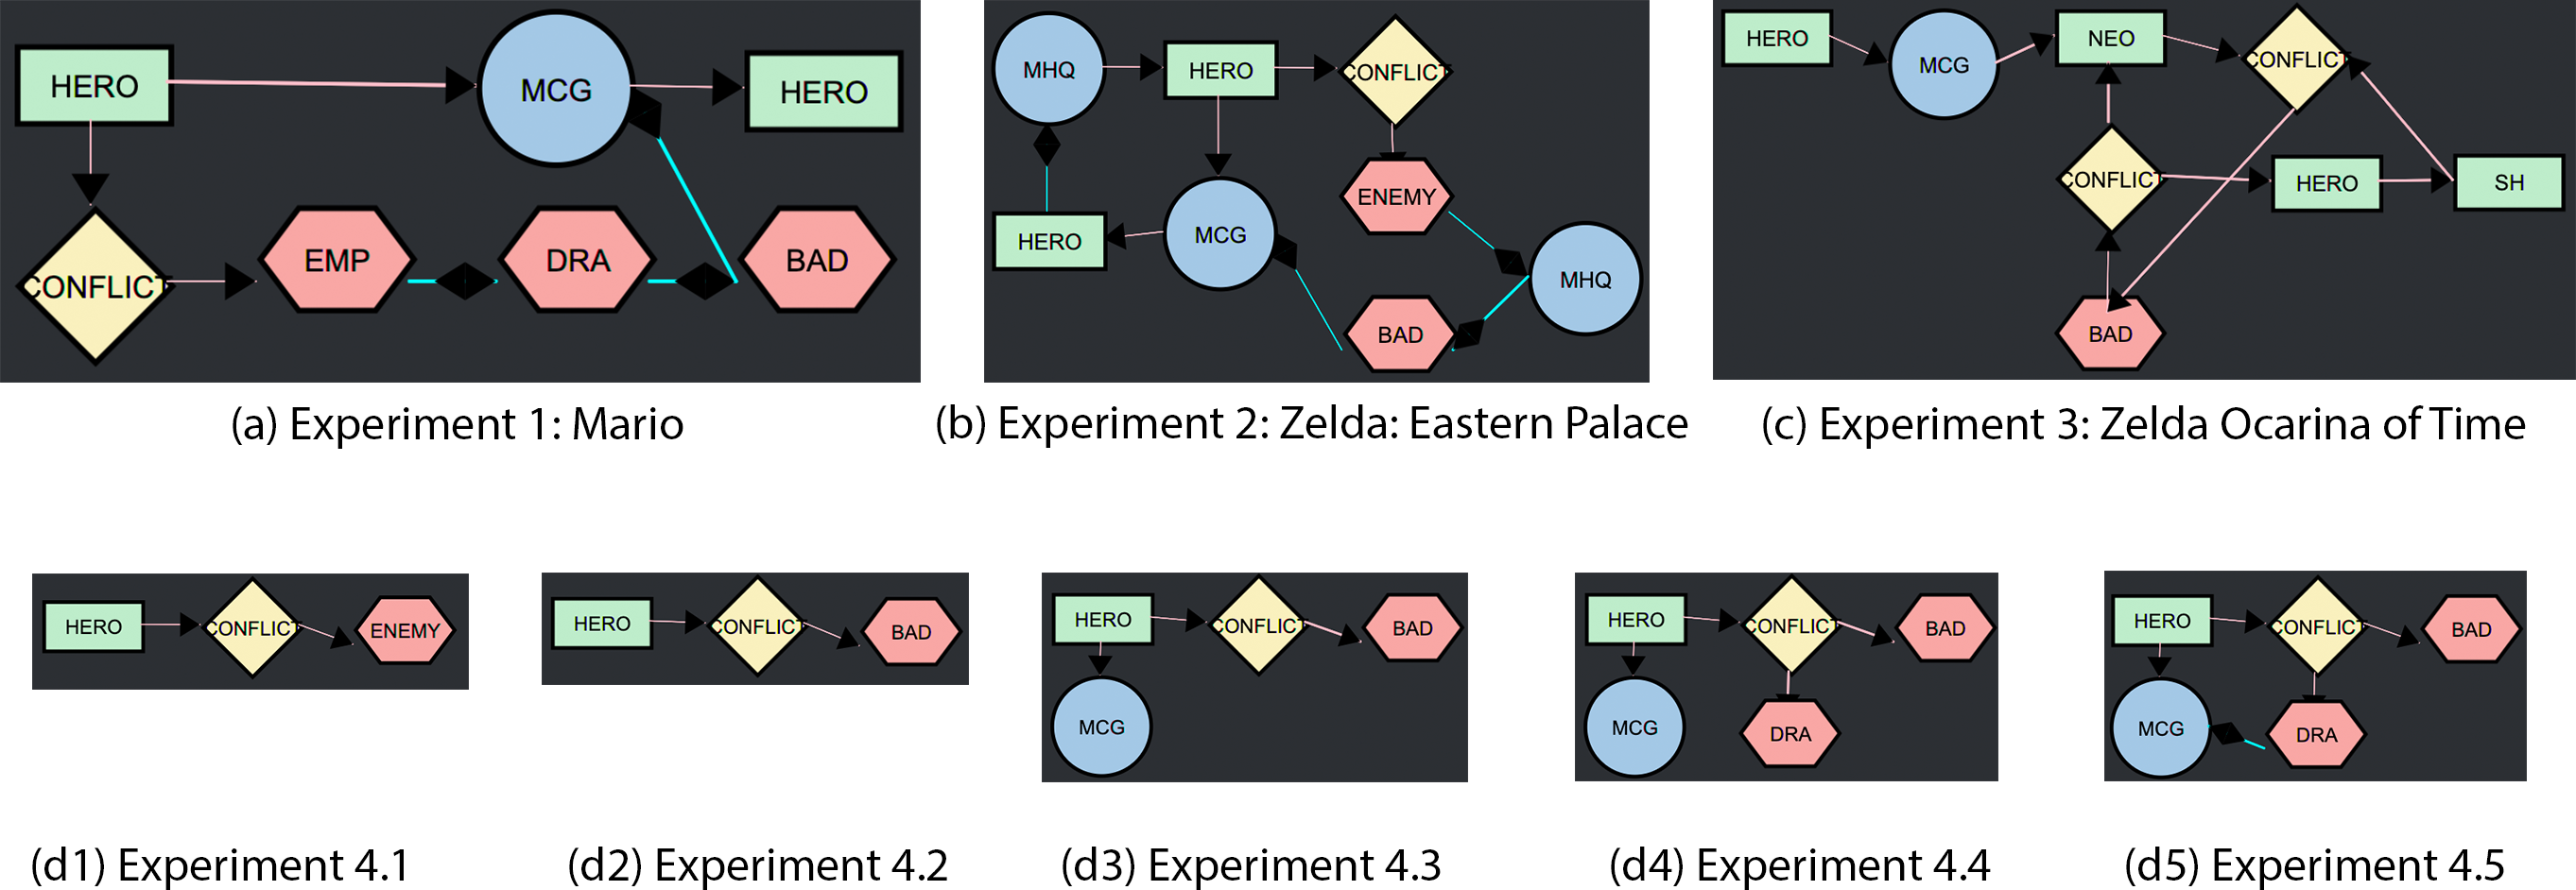
\includegraphics[width=\textwidth]{figures/example-experiments.png}
    \caption{Narrative graphs used for the experiments, constructed and designed in Story Designer. When experiment 4 is discussed, the narrative graph referred is Experiment 4.5 as that is the design's final step.}
    \label{fig:examples}
\end{figure*}

\textbf{Diversity (div).} Diversity measures the variety of [base] trope types within a narrative structure. Currently, there exist four base trope types, \textit{Hero} (h), \textit{Villain} (v), \textit{Structure} (s), \textit{Plot Devices} (pd). Diversity takes into account the tropes that also extend these base tropes. Thus, $D_{div}$ collects all tropes within a graph, and increase a counter for each of the base trope type ($NG_{base} = h, v, s, pd \in NG$), normalized by the max amount of base trope types depicted in Eq.~\ref{eq:diversityDim}:

%\textbf{Diversity (div).} Diversity measures the variety of [base] trope types within a narrative structure. Currently, there exist four base trope types, \textit{Hero} (h), \textit{Villain} (v), \textit{Structure} (s), \textit{Plot Devices} (pd). Diversity takes into account the tropes that also extend these base tropes shown in table~\ref{tab:tropes}. Thus, $D_{div}$ collects all tropes within a graph, and increase a counter for each of the base trope type ($NG_{base} = h, v, s, pd \in NG$), normalized by the max amount of base trope types depicted in Eq.~\ref{eq:diversityDim}:

\begin{equation}
\label{eq:diversityDim}
D_{div} =  \frac{NG_{base}}{\#Trope_{base}}
\end{equation}

%Equation~\ref{eq:diversityDim} shows  is calcula
%A measurement of the variety of trope types included in the graph's nodes in relation to its size.

\textbf{Conflict (confs).} Since we already calculate all patterns within a narrative graph, conflict simply calculates the amount of \emph{explicit} conflict patterns ($\#NG_{c} = C_{exp} \in allPatterns$) that exist within a narrative graph normalized by a conflict threshold $\omega = 5$. We use $\omega$ to avoid stimulating the generation of narrative graphs with a massive amount of conflicts, which could create noise in the evolution and focus on the conflicts rather than other tropes and patterns. $D_{confs}$ is then calculated as $\frac{\#NG_{c}}{\omega}$.

%Equation~\ref{eq:ConfsDim} shows the final calculation of $D_{confs}$.

%\begin{equation}
%\label{eq:ConfsDim}
%D_{confs} =  \frac{\#NG_{c}}{\omega}
%\end{equation}

\textbf{Plot points (pp).} Plot points measures the amount of plot points within a narrative graph ($\#NG_{pp} = pp \in allPatterns$) and normalize it by $\delta$. Given that plot points are dynamically assessed based on other patterns and combination of tropes, we limit the dimension with $\delta$ to avoid losing coherence in favor of generating more plot points. $D_{pp}$ is calculated as $\frac{\#NG_{pp}}{\delta}$.

\textbf{Plot Twist (pt).} Plot twist measures the amount of plot twists within a narrative graph ($\#NG_{pt} = pt \in allPatterns$) and normalize it by $\delta$. Plot twists relate to special situations within a narrative graph where the somewhat abrupt change in the tropes or combination of tropes could alter the narrative and create a surprise effect. Therefore, we limit the dimension with $\delta$ to avoid ``degenerating" narratives with too many twists. $D_{pp}$ is calculated as $\frac{\#NG_{pt}}{\delta}$.

\textbf{Plot devices (pd).} Plot devices measure the amount of active plot devices within a narrative graph ($\#NG_{pd} = apd \in allPatterns$) and normalize it by $\delta$. Plot devices create targets and goals within a narrative, and active plot devices operationalize these in the narrative graph associating them with multiple tropes; thus, similar to \emph{pt}, we limit with $\delta$ to avoid ``degenerating" the narrative. $D_{pd}$ is calculated as $\frac{\#NG_{pd}}{\delta}$.



%How many plot devices are included in the graph in relation to its size

%therefore, we leverage from the \emph{plot point}, \emph{plot twist}, and \emph{active plot device} patterns and the ratio of fake conflicts to measure the \emph{int} of the generated narrative graphs.

%\textbf{Interestingness (int).} With interesting, we aim at measuring the semantic quality of a narrative graph. A narrative graph can be syntactically correct and coherent yet do not have a good (or existent) semantic quality and do not evoke interest for designers and players. Therefore, we leverage from the \emph{plot point}, \emph{plot twist}, and \emph{active plot device} patterns to measure the \emph{int} of the generated narrative graphs. Given that \emph{int} combines these three qualities designers might not be interested in highly\footnote{Interesting-boring qualities are subjective measurements, thus what is highly interesting in our system might not necessarily be for a designer, which is why (in part) we leverage on the narrative graph created by the designer to measure and evaluate patterns and their quality.} interesting generated narrative graphs as they could degrade their narrative objective. Furthermore, the nature of \emph{int} creates pressure on the fitness function since the incidence of the three above-mentioned patterns could (if overused) "degenerate" the narrative; thus, decreasing its coherence. $D_{int}$ is calculated as the weighted sum ($w_{0}=0.4, w_{1}=0.2, w_{2}=0.4$) of the cumulative quality of \emph{plot twists} and \emph{active plot devices} within a narrative graph normalized by their count, and the \emph{plot point} count normalized by the amount of nodes in the graph (equation~\ref{eq:interesting_fitness}).



%\begin{equation}
%\label{eq:fitness}
%f(narrative) = w_{0} * f(interesting) + w_{1} * f(coherence)
%\end{equation}

%The fitness function encompasses a weighted sum between \textit{interest} and \textit{coherence}.


